\documentclass[a4paper,12pt]{article}
% \input{../../../config.tex}
\usepackage{../../../mypackages}
\usepackage{../../../macros}


\usetikzlibrary{shapes,arrows,babel}
\tikzstyle{box}=[minimum size = 0.1cm, rectangle, draw=black, fill=gray]

\def\WITH_CORRECTION{YES}

\begin{document}

\title{Fonctions - Rappels de 2nde}
\author{N. Bancel}

\sloppy  % This will apply the sloppy setting to the entire document.
\maketitle

\section{Vocabulaire des fonctions - Fonctions affines}

\begin{enumerate}
  \item A chaque nombre réel \(x\) d'un intervalle \(I\), une fonction \(f\) associe un nombre réel et un seul que l'on note \(f(x)\). Qu'est ce qu'une image ? Qu'est-ce que l'ensemble de définition ? Qu'est qu'un antécédent ? \par
  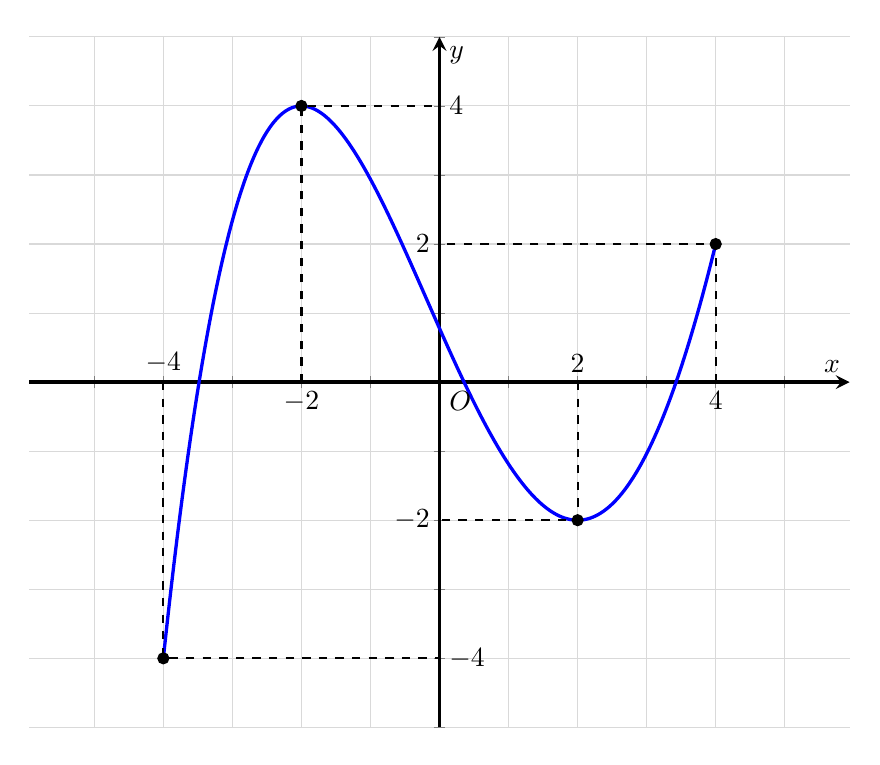
\begin{tikzpicture}[
    declare function={
        f(\x)=-(1/72)*\x^4+3/16*(\x^3)+(1/9)*\x^2-9/4*\x+7/9;
    }
    ]
    \begin{axis}[axis equal,
    width=12 cm, 
    grid=major, 
    axis x line=middle, axis y line=middle,
    axis line style = very thick,
    grid style={gray!30},
    ymin=-5, ymax=5, yticklabels={}, ylabel=$y$,
    xmin=-5, xmax=5, xticklabels={}, xlabel=$x$,
    samples=500,
    ]
    \addplot[blue, very thick,domain=-4:4, smooth]{f(x)};
    \node[below] at (-2, 0) {$-2$};
    \node[above ] at (-4, 0) {$-4$};
    \node[below ] at (4, 0) {$4$};
    \node[right] at (0,-4) {$-4$};
    \node[left  ] at (0,2) {$2$};
    \node[ right ] at (0,4) {$4$};
    \node[below right] at (0, 0) {$O$};
    \node[above ] at ( 2,0) {$2$};
    \node[left  ] at (0, -2) {$-2$};
    \addplot [mark=*,only marks,samples at={-4,-2,2,4}] {f(x)};
    ;
    \draw[dashed, thick] (-4,0) -- (-4,-4) -- (0,-4);
    \draw[dashed, thick] (-2,0) -- (-2,4) -- (0,4);
    \draw[dashed, thick] (2,0) -- (2,-2) -- (0,-2);
    \draw[dashed, thick] (4,0) -- (4,2) -- (0,2);
    \end{axis}
    \end{tikzpicture}
  \ans{
  }{5}{FALSE}
\end{enumerate}

\end{document}
